% High-level layered architecture (Section 3.1).
\documentclass[tikz,border=1pt]{standalone}
% =====================================================================
%  Shared style for every diagram in the proposal.
%  Each figure is a standalone TikZ file that \input's this preamble, so
%  all diagrams use the same font family (Computer Modern, T1 -- identical
%  to the LLNCS body text), the same sizes and the same palette.
%
%  Font rule (do not change per figure):
%    node text   \footnotesize  (8 pt)
%    edge labels \scriptsize    (7 pt)
%    titles      \footnotesize\bfseries
%  Figures are drawn at their final width (<= 12.2 cm, the LLNCS text
%  width) and included WITHOUT scaling, so the printed size is the same
%  in every figure.
% =====================================================================
\usepackage[T1]{fontenc}
\usepackage{amsmath,amssymb}
\usepackage{xcolor}
\usepackage{tikz}
\usetikzlibrary{positioning,arrows.meta,shapes.geometric,shapes.multipart,
  fit,backgrounds,calc,shadows,patterns}

% ---- palette ---------------------------------------------------------
\definecolor{cBlue}{HTML}{0B4F8A}    % application / API
\definecolor{cOrange}{HTML}{B4540A}  % processing / services
\definecolor{cPurple}{HTML}{5B3CC4}  % data stores
\definecolor{cGreen}{HTML}{1B7A3A}   % success / output
\definecolor{cRed}{HTML}{B42318}     % error / risk
\definecolor{cGray}{HTML}{5F6672}    % external / neutral
\definecolor{cInk}{HTML}{1F2933}     % text and arrows

\colorlet{fBlue}{cBlue!9}
\colorlet{fOrange}{cOrange!10}
\colorlet{fPurple}{cPurple!9}
\colorlet{fGreen}{cGreen!10}
\colorlet{fRed}{cRed!9}
\colorlet{fGray}{cGray!8}

% ---- fonts -----------------------------------------------------------
\newcommand{\figfont}{\footnotesize}
\newcommand{\lblfont}{\scriptsize}
\newcommand{\code}[1]{\texttt{#1}}

\tikzset{
  every picture/.style={font=\figfont, line join=round, >={Stealth[length=4pt,width=3.4pt]}},
  every node/.append style={execute at begin node={\hyphenpenalty=10000\exhyphenpenalty=10000}},
  base/.style={draw, rounded corners=2pt, line width=0.6pt, align=center,
               inner xsep=3pt, inner ysep=2.5pt, text=cInk, font=\figfont},
  app/.style={base, draw=cBlue, fill=fBlue},
  svc/.style={base, draw=cOrange, fill=fOrange},
  data/.style={base, draw=cPurple, fill=fPurple},
  ok/.style={base, draw=cGreen, fill=fGreen},
  bad/.style={base, draw=cRed, fill=fRed},
  ext/.style={base, draw=cGray, fill=fGray},
  plain/.style={base, draw=none, fill=none},
  db/.style={cylinder, shape border rotate=90, aspect=0.22, draw=cPurple,
             fill=fPurple, line width=0.6pt, align=center, text=cInk,
             minimum height=9mm, font=\figfont},
  decision/.style={diamond, aspect=2.2, draw=cOrange, fill=fOrange,
                   line width=0.6pt, align=center, inner sep=1pt, text=cInk, font=\figfont},
  actor/.style={draw=cInk, fill=fGray, line width=0.8pt, rounded corners=0pt,
                align=center, inner sep=3pt, font=\figfont\bfseries},
  layer/.style={draw=cGray!60, fill=cGray!4, rounded corners=3pt, line width=0.5pt},
  layertitle/.style={font=\lblfont\bfseries, text=cGray, anchor=north west, inner sep=2pt},
  arr/.style={->, draw=cInk, line width=0.6pt},
  darr/.style={->, draw=cGray, line width=0.6pt, dashed},
  biarr/.style={<->, draw=cInk, line width=0.6pt},
  lbl/.style={font=\lblfont, text=cInk, inner sep=1.5pt},
  lblbg/.style={font=\lblfont, text=cInk, inner sep=1.5pt, fill=white},
}

% ---- UML sequence-diagram helpers -----------------------------------
%  \lifeline{id}{x}{label}{bottom y}   head box + dashed life line
%  \msg{x1}{x2}{y}{label}              synchronous call (solid)
%  \ret{x1}{x2}{y}{label}              reply (dashed)
%  \selfmsg{x}{y}{label}               call to self, label on the right
%  \fragment{kind}{guard}{x1}{y1}{x2}{y2}  combined fragment (alt/loop/par)
\newcommand{\lifeline}[4]{%
  \node[app, text width=19mm, minimum height=8.5mm, font=\figfont\bfseries] (#1) at (#2,0) {#3};
  \draw[cGray, dashed, line width=0.5pt] (#1.south) -- (#2,#4);}
\newcommand{\msg}[4]{%
  \draw[arr] (#1,#3) -- node[lbl, above] {#4} (#2,#3);}
\newcommand{\ret}[4]{%
  \draw[darr] (#1,#3) -- node[lbl, above] {#4} (#2,#3);}
\newcommand{\selfmsg}[3]{%
  \draw[arr] (#1,#2+0.12) -- ++(0.3,0) -- ++(0,-0.24) -- ++(-0.3,0);
  \node[lbl, anchor=west, align=left] at (#1+0.35,#2) {#3};}
\newcommand{\fragment}[6]{%
  \draw[cGray, line width=0.5pt] (#3,#4) rectangle (#5,#6);
  \node[anchor=north west, draw=cGray, fill=white, font=\lblfont\bfseries,
        inner sep=1.5pt, line width=0.5pt] at (#3,#4) {#1};
  \if\relax\detokenize{#2}\relax\else
  \node[anchor=north west, font=\lblfont, text=cGray, inner sep=1.5pt] at (#3+0.75,#4) {[#2]};\fi}
\newcommand{\activation}[3]{% x, y top, y bottom
  \draw[draw=cBlue, fill=fBlue, line width=0.5pt] (#1-0.07,#2) rectangle (#1+0.07,#3);}

\begin{document}
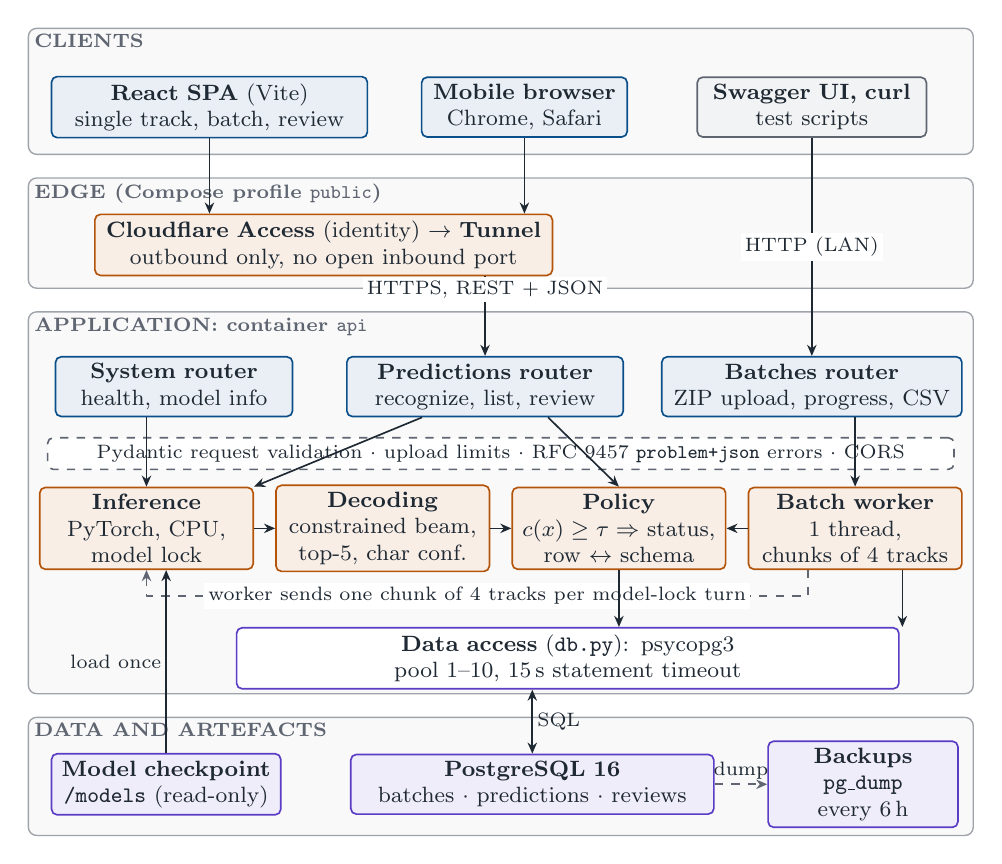
\begin{tikzpicture}
  % ---------------- bands ----------------
  \draw[layer] (0,0)     rectangle (12,-1.6);
  \node[layertitle] at (0,0) {CLIENTS};
  \draw[layer] (0,-1.9)  rectangle (12,-3.3);
  \node[layertitle] at (0,-1.9) {EDGE (Compose profile \code{public})};
  \draw[layer] (0,-3.6)  rectangle (12,-8.45);
  \node[layertitle] at (0,-3.6) {APPLICATION: container \code{api}};
  \draw[layer] (0,-8.75) rectangle (12,-10.25);
  \node[layertitle] at (0,-8.75) {DATA AND ARTEFACTS};

  % ---------------- clients ----------------
  \node[app, text width=38mm] (spa) at (2.3,-1.0) {\textbf{React SPA} (Vite)\\single track, batch, review};
  \node[app, text width=24mm] (mob) at (6.3,-1.0) {\textbf{Mobile browser}\\Chrome, Safari};
  \node[ext, text width=27mm] (cli) at (9.95,-1.0) {\textbf{Swagger UI, curl}\\test scripts};

  % ---------------- edge ----------------
  \node[svc, text width=56mm] (edge) at (3.75,-2.75)
    {\textbf{Cloudflare Access} (identity) $\rightarrow$ \textbf{Tunnel}\\outbound only, no open inbound port};

  % ---------------- application ----------------
  \node[app, text width=28mm] (rsys) at (1.85,-4.55) {\textbf{System router}\\health, model info};
  \node[app, text width=33mm] (rpre) at (5.8,-4.55) {\textbf{Predictions router}\\recognize, list, review};
  \node[app, text width=36mm] (rbat) at (9.95,-4.55) {\textbf{Batches router}\\ZIP upload, progress, CSV};
  \node[base, draw=cGray, dashed, fill=white, text width=113mm, font=\lblfont] (mw) at (6,-5.4)
    {Pydantic request validation $\cdot$ upload limits $\cdot$ RFC 9457 \code{problem+json} errors $\cdot$ CORS};
  \node[svc, text width=25mm] (inf) at (1.5,-6.35)  {\textbf{Inference}\\PyTorch, CPU,\\model lock};
  \node[svc, text width=25mm] (dec) at (4.5,-6.35)  {\textbf{Decoding}\\constrained beam,\\top-5, char conf.};
  \node[svc, text width=25mm] (pol) at (7.5,-6.35)  {\textbf{Policy}\\$c(x)\ge\tau\Rightarrow$ status,\\row $\leftrightarrow$ schema};
  \node[svc, text width=25mm] (wrk) at (10.5,-6.35) {\textbf{Batch worker}\\1 thread,\\chunks of 4 tracks};
  \node[base, draw=cPurple, fill=white, text width=82mm] (dal) at (6.85,-8.0)
    {\textbf{Data access} (\code{db.py}): psycopg3 pool 1--10, 15\,s statement timeout};

  % ---------------- data ----------------
  \node[data, text width=27mm] (ckpt) at (1.75,-9.6) {\textbf{Model checkpoint}\\\code{/models} (read-only)};
  \node[data, text width=44mm] (pg) at (6.4,-9.6) {\textbf{PostgreSQL 16}\\batches $\cdot$ predictions $\cdot$ reviews};
  \node[data, text width=22mm] (bak) at (10.6,-9.6) {\textbf{Backups}\\\code{pg\_dump} every 6\,h};

  % ---------------- flows ----------------
  \draw[arr] (spa.south) -- (spa.south |- edge.north);
  \draw[arr] (mob.south) -- (mob.south |- edge.north);
  \draw[arr] (edge.south -| rpre.north) -- node[lblbg, pos=0.17] {HTTPS, REST + JSON} (rpre.north);
  \draw[arr] (cli.south) -- node[lblbg, pos=0.5] {HTTP (LAN)} (cli.south |- rbat.north);

  \draw[arr] ([xshift=-8mm]rpre.south) -- (inf.north east);
  \draw[arr] ([xshift=8mm]rpre.south) -- (pol.north);
  \draw[arr] (rbat.south -| wrk.north) -- (wrk.north);
  \draw[arr] (rsys.south -| inf.north) -- (inf.north);
  \draw[arr] (inf) -- (dec);
  \draw[arr] (dec) -- (pol);
  \draw[arr] (wrk) -- (pol);
  \draw[darr] ([xshift=-6mm]wrk.south) -- ++(0,-0.33) -| node[lblbg, pos=0.25] {worker sends one chunk of 4 tracks per model-lock turn} (inf.south);
  \draw[arr] (pol.south) -- (pol.south |- dal.north);
  \draw[arr] ([xshift=6mm]wrk.south) -- ([xshift=6mm]wrk.south |- dal.north);
  \draw[biarr] (pg.north |- dal.south) -- node[lbl, right] {SQL} (pg.north);
  \draw[arr] (ckpt.north) -- node[lbl, left, pos=0.5] {load once} (ckpt.north |- inf.south);
  \draw[darr] (pg) -- node[lbl, above] {dump} (bak);
\end{tikzpicture}
\end{document}
